\documentclass[11pt]{apa6}

\usepackage{listings}
\usepackage{graphicx}

\begin{document}
\title{C++ Optimized Linear and Polynomial Regression}
\author{Jarred Parr}
\affiliation{}
\date{January 2019}
\maketitle

\section{Introduction}
Linear regression sits as one of the key introductory problems solved in introductory machine learning coursers, this project is no exception. The goal of this project was the implement linear regression in a unique way that would
hopefully be seen as an improvement over the well-known approaches. C++ was used to compare how the gcc compiler handles advanced implementations. Vector math and other such operations can be computationally intensive. On a
standard Intel CPU with no hyper-threading, I tasked myself with seeing just how much I could squeeze out of this program via analysis of the hot-path and compiler optimization options.

\section{Program Architecture}
Architecturally, many notes were taken from the high-frequency trading practices. Liberal use of the STL was able to promote significant code speedup in some places, especially in the linear trend line case. Observation of this code
particularly around lines 31-37, the long block of const double assignments, shows how powerful the STL has gotten in modern C++. I was able to shrink many cumbersome for loops and hard-to-read expressions into simple and easy to
interpret one-line expressions. The $x^2$ calculation and the $xy$ pair calculations were able to be extremely heavily optimized through the $std::inner_product()$ function. Instead of running nested loops to perform the square
calculation, this code run time remains the same, but the code overhead reduction of taking away the compiler's need to perform inference on what the code is doing allowed for a speedup of about 1.74. This was verified by running
the for-loop implementation against the STL-heavy implementation inside of $godbolt.org$ and also with the Google code profiler. For the polynomial regression, performing the complex linear algebra of acquiring an upper triangular
matrix, then back-substituting the values down the chain is computationally intensive. Great care was taken to remove ambiguity from the compiler to allow it to run as efficiently as possible, but the lack of STL-magic being able
to save me made it hard to optimize heavily. Some routines were scrubbed after inspection in the $godbolt.org$ assembly code inspector and the overall assembly code shrank considerably under gcc's highest optimization $(-O3)$, but
it still only gave a modest speedup of 1.2.

\section{Growth Areas}
Linear algebra, as it stands, is pretty straightforward. Matrix math and computations are not too difficult where it would be unwieldy to the faint of heart, but not too trivial that it is unnecessary to have a grasp of the needed skills. However,
this project sought to stretch my understanding of doing these operations raw (no library support), and in a language like C++, it was definitely a bit of an uphill struggle to say the least. Many times during optimization, especially for my matrix
normalization process, I found that there was a great deal of debugging that had to be done to properly access indices of matrices under certain circumstances. To be more granular, there were many specific cases, like when trying to handle the
detection of upper triangular matrices, which would then trigger the next step in simplifying the linear system. It isn't as simple as saying $if (matrix == identity\_matrix) \{ exit; \}$, instead, guards needed to be implemented to check for $terminal$
conditions or, more simply, a point where the matrix could no longer be simplified. Since not all matrices simplify to the identity matrix, it was tricky to figure out when a particular matrix had the right values, which then allowed me to perform
the needed calculations to acquire the coefficients to the polynomial equation. It definitely took much longer than I had wanted, but it was very enlightening to apply the math advice of my current linear algebra professor to these unique problems.

\section{Managing Data}
Inside of the provided $downloads.txt$ file, a choice had to be made about the handling of the missing fields. I opted to just drop those rows. With the large volume of data, the rows with $NaN$ values was only about 1.2\% of the data. As can be seen below in my results, removing these 4 or 5 columns had no major affect on the output. However, in the event that there were significantly missing fields, imputation would be used to handle this problem. Imputation is the process of filling in likely values in the place of $NaN$ values based on the values around it. Depending on the context, this can be a good or a bad choice for the problem. An example of this would be if you're analyzing social media data, imputation is fine since there isn't much riding on the data being absolutely 100\% accurate. However, in the case of something like medical records, you would ideally just take the data as-is to avoid making any false conclusions.

\section{Source Code}
All source code is provided at the end of this document to maintain formatting.

\section{Results}
\begin{figure}[!htb]
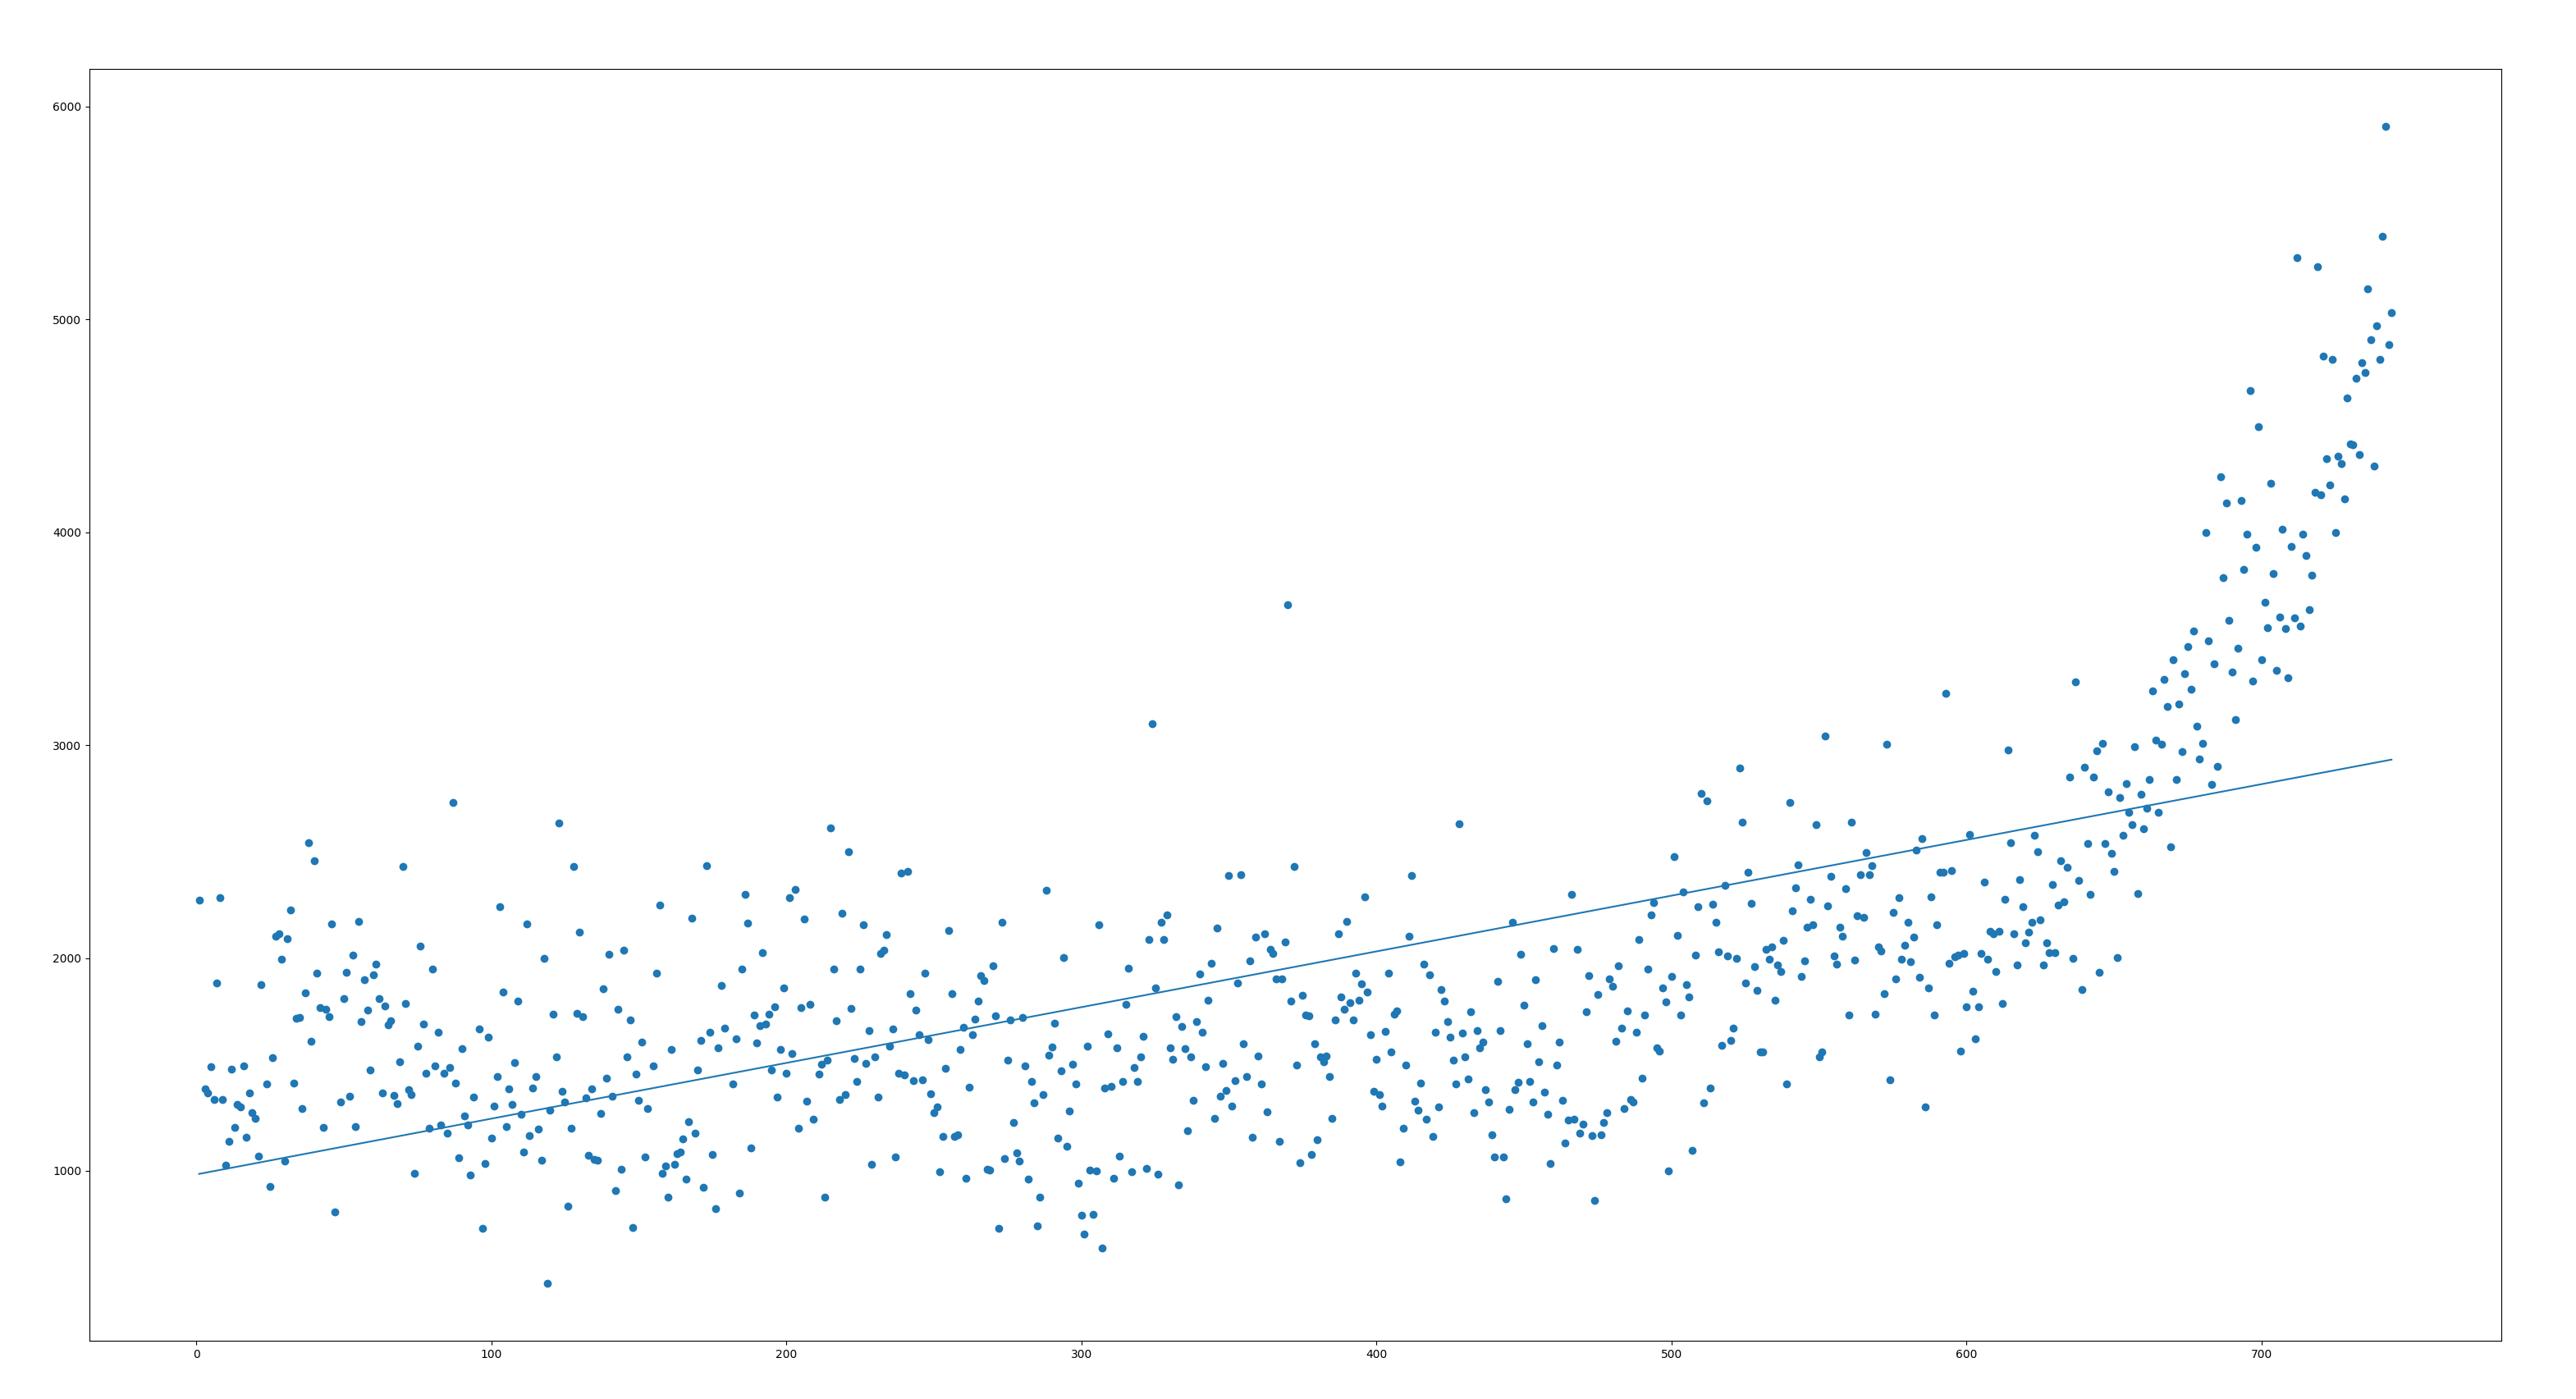
\includegraphics[width=3in]{linreg.png}
\caption{Simple Linear Regression}
\label{fig1}
\end{figure}
The simple linear classifier was easy to implement. As you can see, it is trending upward because of the positive review. I had initially postulated the idea of removing the positive review data to get a true idea of the downloads before the famous
person endorsed the book, however, it is clear that that may not have given an accurate view of what the data is. Without being able to see the data after this point, the book sales could have continued to sell extremely well as thery were previously.
As a result, it was left in the data. For the polynomial regression, you much of the same thing, except with a bit more accurate of a reading of the information. With this information, I was able to determine that the number of sales at noon on the 5th day of the month at noon would be approximately $3238$ books. All results were verified by the scikit-learn python package and matplotlib to ensure my diagrams and equations were accurate.
\begin{figure}[!htb]
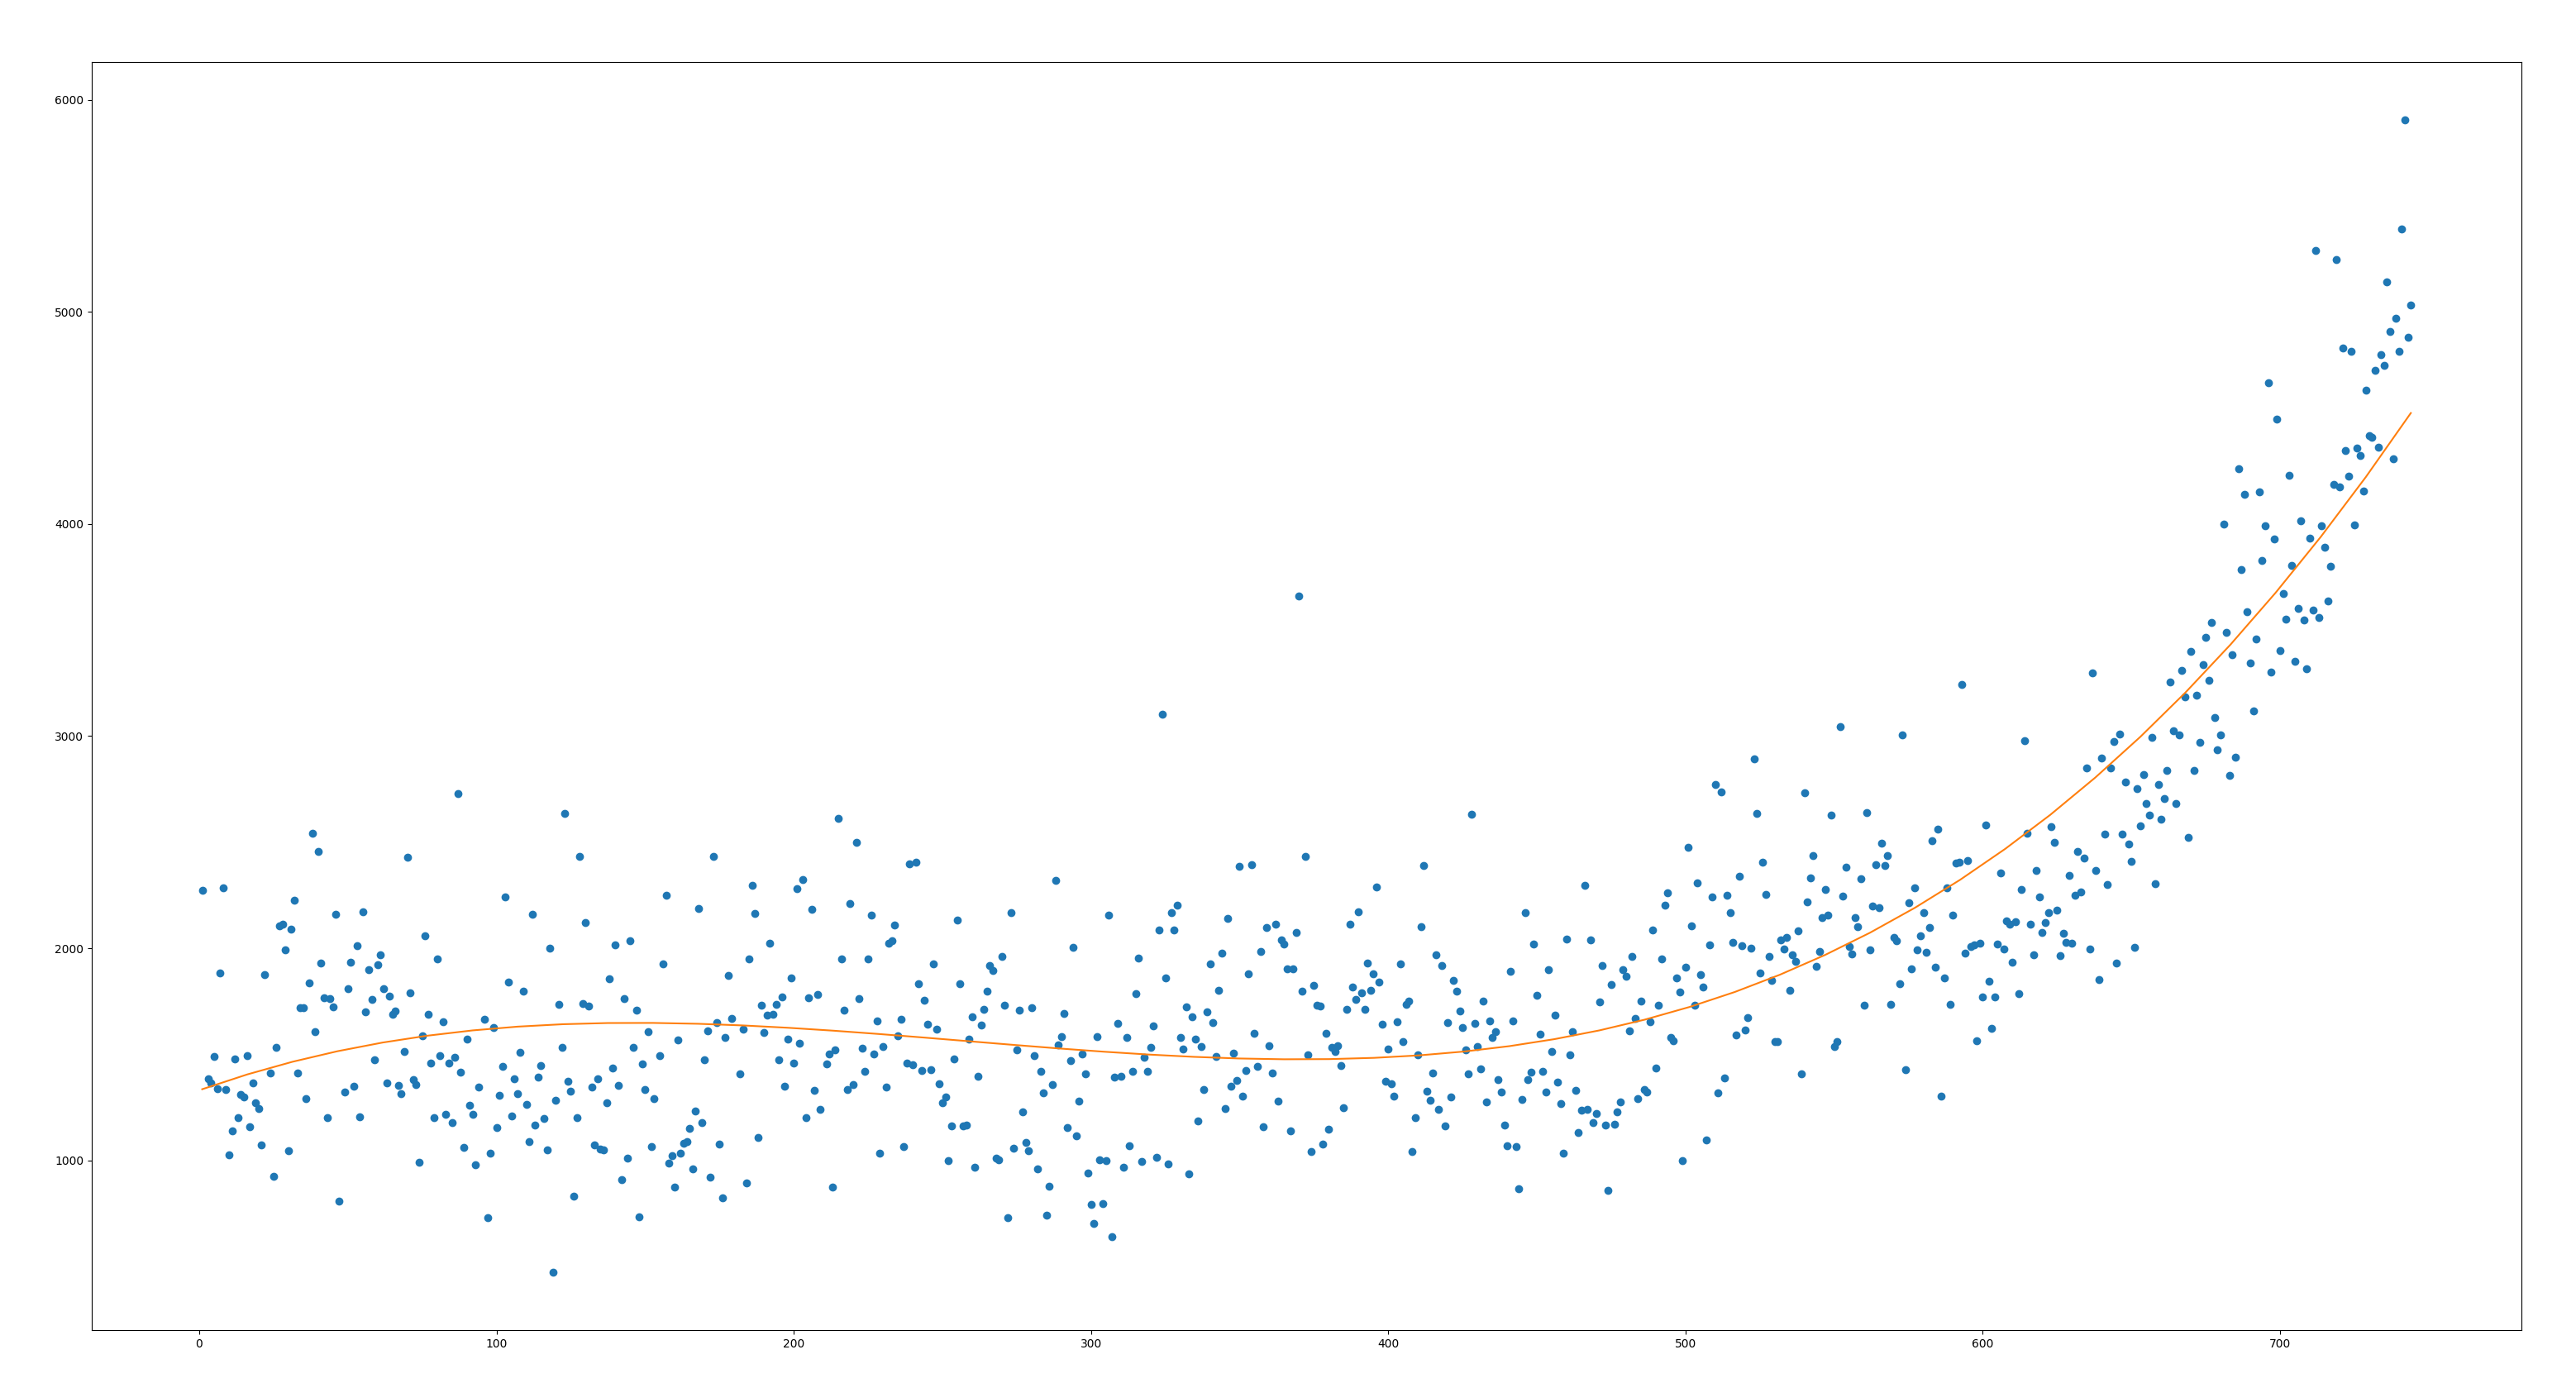
\includegraphics[width=3in]{polynomialreg.png}
\caption{Simple Polynomial Regression}
\label{fig2}
\end{figure}

\section{Conclusion}
This project taught me a lot about micro-optimization. Since Linear Regression is a fairly straightforward process, it can be easy to write it off as simply another frivolous exercise. However, digging into more advanced classification techniques
and expansion areas on the subject at hand can facilitate some interesting results and hypothesis. C++ optimized for smaller-scale regression tasks like this one doesn't truly show the optimization that can be made, however in the case of a
regression of significantly more data, it is clear where the benefits of having such a low-level hardware optimized codebase can shine. There was a significant speedup between instances of STL usage and instances of manual code. It is clear that
when the compiler has less to think about, regression tasks become infinitely quicker to accomplish.
\end{document}
